\section{The Screen Editor}
\label{sec:screen-editor}

When you turn on your MEGA65 or reset it, the following screen will appear:

\begin{center}
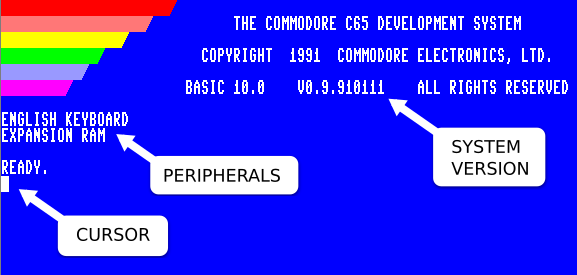
\includegraphics[width={10cm}]{images/introduction-screen/layout.png}
\end{center}

The colour bars in the top left hand of the screen can be used
as a guide to help calibrate the colours of your display.
The screen also displays the name of the system,
the copyright notice, and the ROM version.
The displayed date and time are taken vom the internal RTC
(Real Time Clock), which can be set in the CONFIGURE menu.

Finally, you will see the READY prompt and the flashing cursor.

You can begin typing keys on the keyboard and the characters will be
printed at the cursor position. The cursor itself will advance after
each key press.

You can also produce reverse text or colour bars by holding down the \megakey{CTRL} key and pressing the \megakey{9} key, or the \megakey{R} key. This enters reverse text mode. When this is enabled, you can press and hold the \megakey{Space bar}. While doing so, a white bar will be drawn across the screen.

You can even change the current colour by holding the \megakey{CTRL} key down and pressing a number key (from \megakey{1} to \megakey{8}). For example, if you press and hold the \megakey{CTRL} key, and press \megakey{1}, the colour will change to black. Now, when you hold down the \megakey{Space bar}, a black bar will be drawn. If you continue to change the colour and press the \megakey{Space bar}, you will get an effect similar to the image below:


\begin{center}
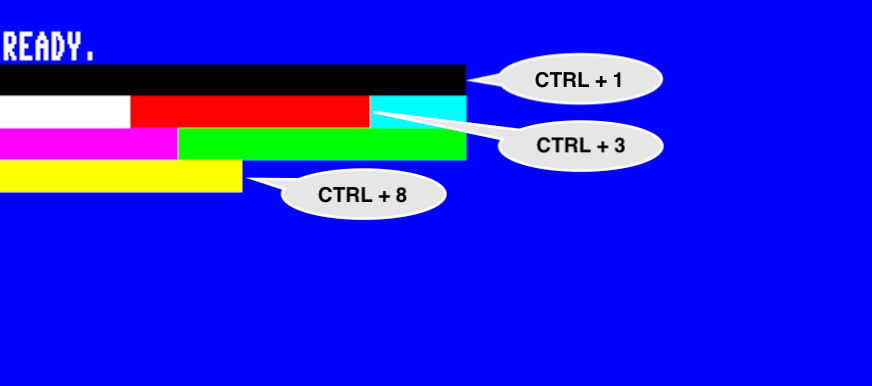
\includegraphics[width={10cm}]{images/introduction-screen/colour-bars.png}
\end{center}


You can disable the reverse text mode by holding \megakey{CTRL} and pressing the \megakey{0} key.

By pressing any keys, the characters will be typed out in the chosen colour.

There are a further eight colours available via the \megasymbolkey key. Hold the \megasymbolkey key and press a key from \megakey{1} to \megakey{8} to change to one of the secondary colours. The colour that is printed at the bottom row on the front of the number key will be used. For example, if you held the \megasymbolkey key down while pressing \megakey{4}, dark green will be used. For even more colours, see \bookvref{appendix:escapesequences}.

\needspace{4cm}
You can create fun pictures just by using these colours and letters.  Here's an example of what a year four student drew:

\begin{center}
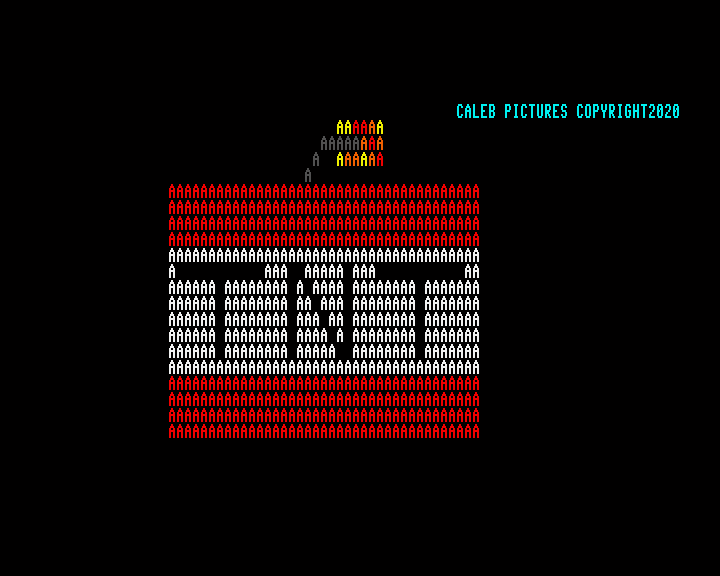
\includegraphics[width={6cm}]{images/caleb-PETSCII-TNT-final}
\end{center}

What will you draw?

\needspace{2cm}
\textbf{Functions}

Functions using the \megakey{CTRL} key are called \textbf{Control Functions}.
Functions using the \megasymbolkey key are called \textbf{Mega Functions}. There are also functions called by using the \megakey{Shift} key. These are (not surprisingly) called \textbf{Shift Functions}.

Lastly, using the \megakey{ESC} key are \textbf{Escape Sequences}.

\needspace{2cm}
\textbf{ESC Sequences}

Escape sequences are performed a little differently than a Control function or a Shifted function. Instead of holding the modifier key down, an Escape sequence is performed by pressing the \megakey{ESC} key and releasing it, followed by pressing the desired key code.

For example: to switch between 40/80 column mode, press and release the \megakey{ESC} key. Then press the \megakey{X} key.

You can see all of the available escape sequences in \bookvref{appendix:escapesequences}, but some are shown in this section.

There are more modes available. You can create flashing text by holding the \megakey{CTRL} key and pressing the \megakey{O} key. Any characters you press will flash. Turn flash mode off by pressing \megakey{ESC} then \megakey{O}.



\section{Editor Functionality}


The MEGA65 screen can allow you to do advanced tabbing, and moving quickly around the screen in many ways to help you to be more productive.

Press the \megakey{Home} key to go to the home position on the screen. Hold the \megakey{CTRL} key down and press the \megakey{W} key several times. This is the \textbf{Word Advance function} which jumps your cursor to the next word, or printable character.

You can set custom tab positions on the screen for your convenience. Press \megakey{Home} and then \megakey{$\rightarrow$} to the fourth column. Hold down \megakey{CTRL} and press the \megakey{X} key to set a tab. Move another 20 positions to the right again, and do \megakey{CTRL} and \megakey{X} again to set a second tab.

Press the \megakey{Home} key to go back to the home position. Hold the \megakey{CTRL} key and press the \megakey{I} key. This is the \textbf{Forward Tab function}. Your cursor will tab to the fourth position. Press \megakey{CTRL} and \megakey{I} again. Your cursor will move to position 8. Why? By default, every 8th position is already set as a tabbed position. So the 4th and 20th positions have been added to the existing tab positions. You can continue to press the \megakey{CTRL} and \megakey{I} keys to the 16th and 20th positions.

To find the complete set of Control codes, see \bookvref{appendix:controlcodes}.

\textbf{Creating a Window}

You can set a window on the MEGA65 working screen. Move your cursor to the beginning of the "BASIC 65" text. Press \megakey{ESC}, then press \megakey{T}. Move the cursor 10 lines down and 15 to the right.

Press the \megakey{ESC} key, then \megakey{B}. Anything you type will be contained within this window.

To escape from the window back to the full screen, press the \megakey{Home} key twice.


\textbf{Extras}

Long press on \megakey{Restore} to go into the Freeze Menu.  Then press \megakey{J} to switch joystick ports without having to physically swap the joystick to the other port.

Go to \textbf{Fast mode} with poke 0, 65 or use the freeze menu.

\megakey{MEGA} and \megakey{Shift} switches between text uppercase and lowercase for the entire display.
